% A LaTeX template for EXECUTIVE SUMMARY of the MSc Thesis submissions to 
% Politecnico di Milano (PoliMi) - School of Industrial and Information Engineering
%
% P. F. Antonietti, S. Bonetti, A. Gruttadauria, G. Mescolini, A. Zingaro
% e-mail: template-tesi-ingind@polimi.it
%
% Last Revision: October 2021
%
% Copyright 2021 Politecnico di Milano, Italy. Inc. All rights reserved.

\documentclass[10.5pt,a4paper,twocolumn]{article}

%------------------------------------------------------------------------------
%	REQUIRED PACKAGES AND  CONFIGURATIONS
%------------------------------------------------------------------------------
% PACKAGES FOR TITLES
\usepackage{titlesec}
\usepackage{color}

% PACKAGES FOR LANGUAGE AND FONT
\usepackage[utf8]{inputenc}
\usepackage[english]{babel}
\usepackage[T1]{fontenc} % Font encoding

% PACKAGES FOR IMAGES
\usepackage{graphicx}
\graphicspath{{Images/}} % Path for images' folder
\usepackage{eso-pic} % For the background picture on the title page
\usepackage{subfig} % Numbered and caption subfigures using \subfloat
\usepackage{caption} % Coloured captions
\usepackage{transparent}

% STANDARD MATH PACKAGES
\usepackage{amsmath}
\usepackage{amsthm}
\usepackage{bm}
\usepackage[overload]{empheq}  % For braced-style systems of equations

% PACKAGES FOR TABLES
\usepackage{tabularx}
\usepackage{longtable} % tables that can span several pages
\usepackage{colortbl}

% PACKAGES FOR ALGORITHMS (PSEUDO-CODE)
\usepackage{algorithm}
\usepackage{algorithmic}

% PACKAGES FOR REFERENCES & BIBLIOGRAPHY
\usepackage[colorlinks=true,linkcolor=black,anchorcolor=black,citecolor=black,filecolor=black,menucolor=black,runcolor=black,urlcolor=black]{hyperref} % Adds clickable links at references
\usepackage{cleveref}
\usepackage[square, numbers, sort&compress]{natbib} % Square brackets, citing references with numbers, citations sorted by appearance in the text and compressed
\bibliographystyle{plain} % You may use a different style adapted to your field

% PACKAGES FOR THE APPENDIX
\usepackage{appendix}

% PACKAGES FOR ITEMIZE & ENUMERATES 
\usepackage{enumitem}

% OTHER PACKAGES
\usepackage{amsthm,thmtools,xcolor} % Coloured "Theorem"
\usepackage{comment} % Comment part of code
\usepackage{fancyhdr} % Fancy headers and footers
\usepackage{lipsum} % Insert dummy text
\usepackage{tcolorbox} % Create coloured boxes (e.g. the one for the key-words)
\usepackage{stfloats} % Correct position of the tables

%-------------------------------------------------------------------------
%	NEW COMMANDS DEFINED
%-------------------------------------------------------------------------
% EXAMPLES OF NEW COMMANDS -> here you see how to define new commands
\newcommand{\bea}{\begin{eqnarray}} % Shortcut for equation arrays
\newcommand{\eea}{\end{eqnarray}}
\newcommand{\e}[1]{\times 10^{#1}}  % Powers of 10 notation
\newcommand{\mathbbm}[1]{\text{\usefont{U}{bbm}{m}{n}#1}} % From mathbbm.sty
\newcommand{\pdev}[2]{\frac{\partial#1}{\partial#2}}
% NB: you can also override some existing commands with the keyword \renewcommand

%----------------------------------------------------------------------------
%	ADD YOUR PACKAGES (be careful of package interaction)
%----------------------------------------------------------------------------


%----------------------------------------------------------------------------
%	ADD YOUR DEFINITIONS AND COMMANDS (be careful of existing commands)
%----------------------------------------------------------------------------


% Do not change Configuration_files/config.tex file unless you really know what you are doing. 
% This file ends the configuration procedures (e.g. customizing commands, definition of new commands)
% Set the geometric layout of the document
\usepackage{geometry}
\geometry{
  top=3cm,
  left = 2.0cm,
  right = 2.0cm,
  bottom=2cm,
  headheight= 2cm,
  headsep= 0cm,
}
\raggedbottom 

% Create color bluePoli (-> manuale grafica coordinata:  https://www.polimi.it/fileadmin/user_upload/il_Politecnico/grafica-coordinata/2015_05_11_46xy_manuale_grafica_coordinata.pdf)
\definecolor{bluePoli}{cmyk}{0.4,0.1,0,0.4}

% Custom theorem environments
\declaretheoremstyle[
  headfont=\color{bluePoli}\normalfont\bfseries,
  bodyfont=\color{black}\normalfont\itshape,
]{colored}

\captionsetup[figure]{labelfont={color=bluePoli}} % Set colour of the captions
\captionsetup[table]{labelfont={color=bluePoli}} % Set colour of the captions
\captionsetup[algorithm]{labelfont={color=bluePoli}} % Set colour of the captions

\theoremstyle{colored}
\newtheorem{theorem}{Theorem}[section]
\newtheorem{proposition}{Proposition}[section]

% Enhances the features of the standard "table" and "tabular" environments.
\newcommand\T{\rule{0pt}{2.6ex}}
\newcommand\B{\rule[-1.2ex]{0pt}{0pt}}

% Algorithm description
\newcounter{algsubstate}
\renewcommand{\thealgsubstate}{\alph{algsubstate}}
\newenvironment{algsubstates}{
    \setcounter{algsubstate}{0}%
    \renewcommand{\STATE}{%
    \stepcounter{algsubstate}%
    \Statex {\small\thealgsubstate:}\space}
    }{}
    
% Custom theorem environment
\newcolumntype{L}[1]{>{\raggedright\let\newline\\\arraybackslash\hspace{0pt}}m{#1}}
\newcolumntype{C}[1]{>{\centering\let\newline\\\arraybackslash\hspace{0pt}}m{#1}}
\newcolumntype{R}[1]{>{\raggedleft\let\newline\\\arraybackslash\hspace{0pt}}m{#1}}

% Custom itemize environment
\setlist[itemize,1]{label=$\bullet$}
\setlist[itemize,2]{label=$\circ$}
\setlist[itemize,3]{label=$-$}
\setlist{nosep}

% Set separation of columns 
\setlength{\columnsep}{30pt}

% Create command for background pic
\newcommand\BackgroundPic{% Adding background picture
	\put(230,358){
		\parbox[b][\paperheight]{\paperwidth}{%
			\vfill
			\centering
			\transparent{0.4}
			
\includegraphics[width=0.5\paperwidth]{raggiera_polimi.eps}%
			\vfill
}}}

% Set indentation
\setlength\parindent{0pt}

% Custom title commands
\titleformat{\section}
{\color{bluePoli}\normalfont\Large\bfseries}
{\color{bluePoli}\thesection.}{1em}{}
\titlespacing*{\section}
{0pt}{2ex}{1ex}

\titleformat{\subsection}
{\color{bluePoli}\normalfont\large\bfseries}
{\color{bluePoli}\thesubsection.}{1em}{}
\titlespacing*{\subsection}
{0pt}{2ex}{1ex}

% Custom headers and footers
\pagestyle{fancy}
\fancyhf{}
      
\fancyfoot{}
\fancyfoot[C]{\thepage} % page
\renewcommand{\headrulewidth}{0mm} % headrule width
\renewcommand{\footrulewidth}{0mm} % footrule width

\makeatletter
\patchcmd{\headrule}{\hrule}{\color{black}\hrule}{}{} % headrule
\patchcmd{\footrule}{\hrule}{\color{black}\hrule}{}{} % footrule
\makeatother

% -> Create the header
%\chead[C]{
%\centering
%\begin{tcolorbox}[arc=0pt, boxrule=0pt, colback=bluePoli!60, width=\textwidth, colupper=white]
%    \textbf{Executive summary} \hfill \textbf{\author}  
%\end{tcolorbox}
%}

% Insert here the info that will be displayed into your Title page 
% -> title of your work
\renewcommand{\title}{Homework 2: Time Series Forecasting}
% -> author name and surname
\renewcommand{\author}{ - Domenico Cacace \\  - Miguel Gonzalez \\  - Usevalad Milasheuski}
\renewcommand{\advisor}{DMU}


%-------------------------------------------------------------------------
%	BEGIN OF YOUR DOCUMENT
%-------------------------------------------------------------------------
\begin{document}

%-----------------------------------------------------------------------------
% TITLE PAGE
%-----------------------------------------------------------------------------
% Do not change Configuration_files/TitlePage.tex (Modify it IF AND ONLY IF you need to add or delete the Co-advisors)
% This file creates the Title Page of the document
% DO NOT REMOVE SPACES BETWEEN LINES!

\twocolumn[{\begin{@twocolumnfalse}

\AddToShipoutPicture*{\BackgroundPic}

\hspace{-0.6cm}
\includegraphics[width=0.6\textwidth]{logo_polimi_ing_indinf.eps}

\vspace{-1mm}
\fontsize{0.3cm}{0.5cm}\selectfont \bfseries \textsc{\color{bluePoli} Artificial Neural Networks and Deep Learning}\\

\vspace{-0.2cm}
\Large{\textbf{\color{bluePoli}{\title}}}\\

%\vspace{-0.2cm}
%\fontsize{0.3cm}{0.5cm}\selectfont \bfseries \textsc{\color{bluePoli} Laurea Magistrale in \course}\\

\vspace{-0.2cm}
\fontsize{0.3cm}{0.5cm} \selectfont \bfseries Authors: \\\textsc{\textbf{\author}}\\

\vspace{-0.4cm}
\fontsize{0.3cm}{0.5cm}\selectfont \bfseries Team name: \textsc{\textbf{\advisor}}\\


% if only ONE co-advisor is present:
%\vspace{-0.4cm}
%\fontsize{0.3cm}{0.5cm}\selectfont \bfseries Co-advisor: \textsc{\textbf{\firstcoadvisor}}\\
% if more than one co-advisors are present:
%\vspace{-0.4cm}
%\fontsize{0.3cm}{0.5cm}\selectfont \bfseries Co-advisors: \textsc{\textbf{\firstcoadvisor}}\textsc{\textbf{\secondcoadvisor}}\\

%\vspace{-0.4cm}
%\fontsize{0.3cm}{0.5cm}\selectfont \bfseries Academic year: \textsc{\textbf{\YEAR}}

\small \normalfont

%\vspace{11pt}

\centerline{\rule{1.0\textwidth}{0.4pt}}

\vspace{15pt}
\end{@twocolumnfalse}}]

\thispagestyle{plain} % In order to not show the header in the first page

%%%%%%%%%%%%%%%%%%%%%%%%%%%%%%
%%     THESIS MAIN TEXT     %%
%%%%%%%%%%%%%%%%%%%%%%%%%%%%%%

%-----------------------------------------------------------------------------
% INTRODUCTION
%-----------------------------------------------------------------------------
\section{Introduction}
\label{sec:introduction}
Our strategy for this homework is to start with simple Recurrent Neural Networks,
evaluating pros and cons of different architectures. Afterwards we implement a 
seq2seq model, on which we can then test \textit{novel} methodologies, such as 
the Luong attention mechanism.\\

\section{Dataset}
\label{sec:dataset}
The dataset used in this project consists of 7 time series, each containing 68529 samples.
As for preprocessing, we normalized the data (MinMax normalization) and extracted the
sequences to be fed to the network with a sliding window approach; 
for our models, we found that a window size of 200 and a stride of 5
yield the best results.\\
The models submitted to the competition are trained on the whole dataset, with a 80/20 split between
training and validation; to determine the performance of a model (based on how well they predict the future) 
and decide what models to submit we reserved  $\sim$15\% of the original dataset for testing.\\
We evaluated both oneshot and autoregressive predictions on most of our model, and found that the
latter produced better predictions in almost all the cases.


\section{Recurrent neural networks}
\label{sec:lstm_gru}
As a first step, we evaluated the different recurrent layers that Keras offers.
For the sake of consistency, we used the same model structure, consisting of:
\begin{itemize}
    \item Recurrent layer(s)
    \item \texttt{Dense} layer
    \item \texttt{Reshape} layer
    \item \texttt{Conv1D} layer
\end{itemize}

For the recurrent layers we used \texttt{LSTM} and \texttt{GRU};
we did not consider at all the \texttt{SimpleRNN} layer, due to its vanishing gradient issue.
We trained our models using the Mean Absolute Error and the Mean Squared Error as accuracy and loss 
functions respectively (we also tried RMSE as loss, and noticed no significant change).
In addition, we employed early stopping (max 200 epochs) and learning rate reduction.

Tests with \textit{unidirectional} layers yielded similar results (RMSE around 9.5) for both LSTM and GRU layers;
changing the number of units per layer (50, 100, 256) and the number of layers (2, 3, 4) did not 
bring a significant improvements. During this phase we observed that, in some cases, there was
a jump discontinuity between the last input and the first predicted value: to solve this issue
we employed a dropout layer after every recurrent one, and observed that the gap disappeared.

\begin{figure}[h]
    \centering
    \begin{minipage}[b]{0.45\linewidth}
        \centering
        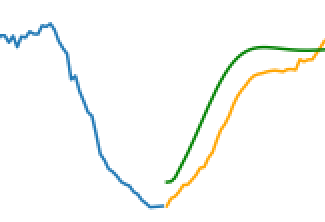
\includegraphics[width=0.8\textwidth]{pics/nodropout.png} % first figure itself
        \caption{no dropout}
    \end{minipage}\hfill
    \begin{minipage}[b]{0.45\linewidth}
        \centering
        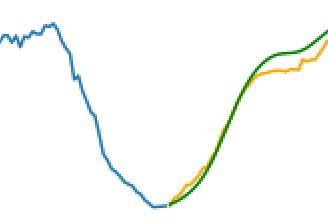
\includegraphics[width=0.8\textwidth]{pics/withdropout.png} % second figure itself
        \caption{dropout (0.2)}
    \end{minipage}
\end{figure}
\newpage
\subsection{Bidirectional layers}
With bidirectional layers we observed significant differences among the models tested;
as above, we changed the number of units per layer and the number of recurrent layers.
We observed that the BiGRU models had significantly worse performances than BiLSTM ones 
for every variation tested: we attributed these outcomes to the structure of the memory
units, as GRUs have less parameters than LSTM units.\\
Regarding BiLSTM models, we obtained the best results with 3 recurrent layers (RMSE 4.0945), while increasing 
the number of layers yields slightly worse results (RMSE 5.1252).
\begin{figure}[h]
    \centering
    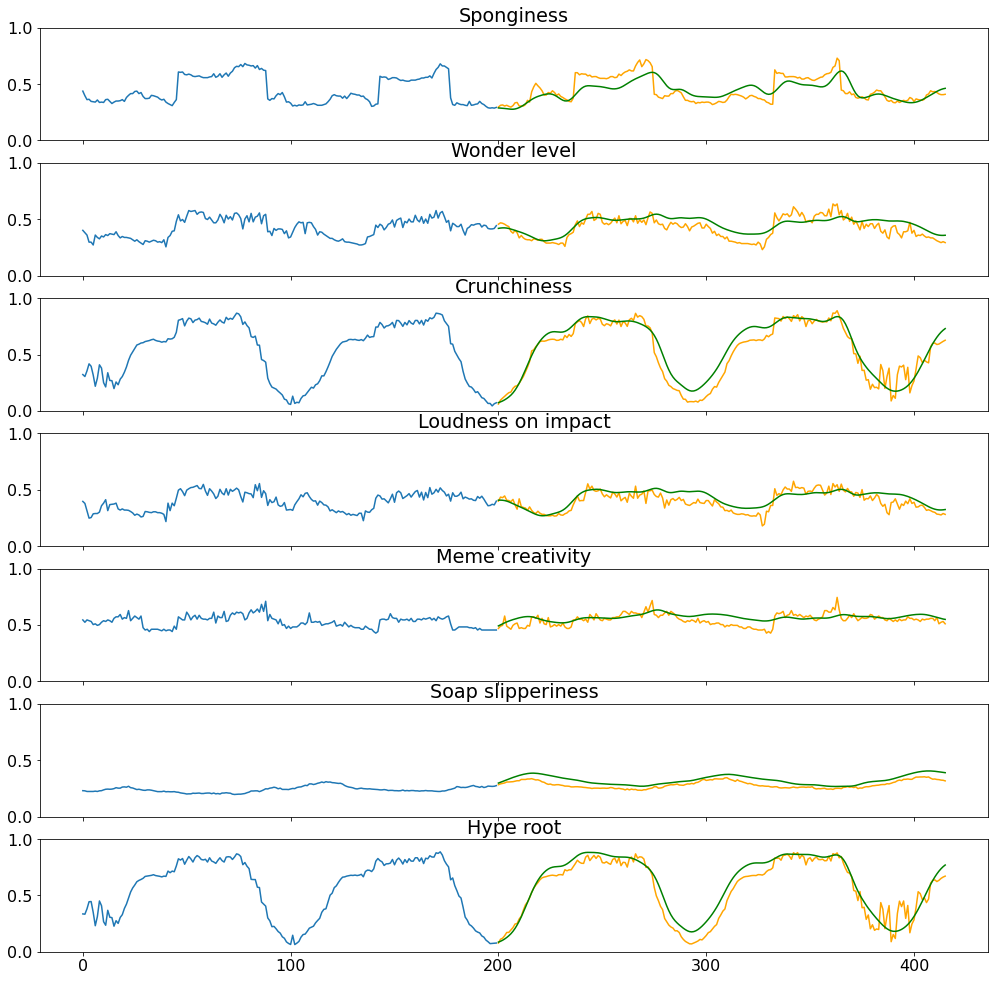
\includegraphics[width=\linewidth]{pics/pred_BiLSTM.png}
    \caption{3 BiLSTM layers (256 units), 0.2 Dropout}
\end{figure}

\section{To seq2seq and beyond}
\label{seq2seq}
\textbf{Disclaimer:} all the models presented in this section have been 
developed during the Codalab outage; the results we got via cross validation
on our local test set differ significantly from the ones we got on the secret test set.\\

Our next step consists in building an encoder/decoder model. Instead of starting from 
scratch, we employed the results obtained in the previous experiments; following the
classic encoder/decoder structure, we have:
\begin{itemize}
    \item 3 BiLSTM layers, for the encoder
    \item 1 \texttt{RepeatVector}, to \textit{connect the components}
    \item 2 BiLSTM layers, for the decoder
    \item 1 \texttt{TimeDistributed} Dense output layer
\end{itemize}

The results on the local test set suggested that this model performed similarly to the 
3-layer BiLSTM; however, this model performs way worse (RMSE 9.7349): by taking a closer look
at the results, we can see that the RMSE quickly diverges as we go \textit{deeper} in the
secret test set, going from 3.86 to 10.29 by moving from the first to the second quarter.

\subsection{Luong attention}
As a final step, we implemented the Luong attention mechanism; in this phase we had
some trouble with the \texttt{Attention} layer provided by Keras, so we implemented
it manually with dot products and Softmax (see the code and the model scheme in the appendix for more details).

By looking at the predictions on the local test set it looks like this model can outperform the 3-layer BiLSTM one,
but the results on the secret test set say otherwise, showing a RMSE of 4.8321. Even though this isn't our best model,
we were able to significantly improve the performance, keeping the RMSE lower among the whole secret test set 
(3.56, 4.59, 6.03 for the three quarters respectively).

\begin{figure}[h]
    \centering
    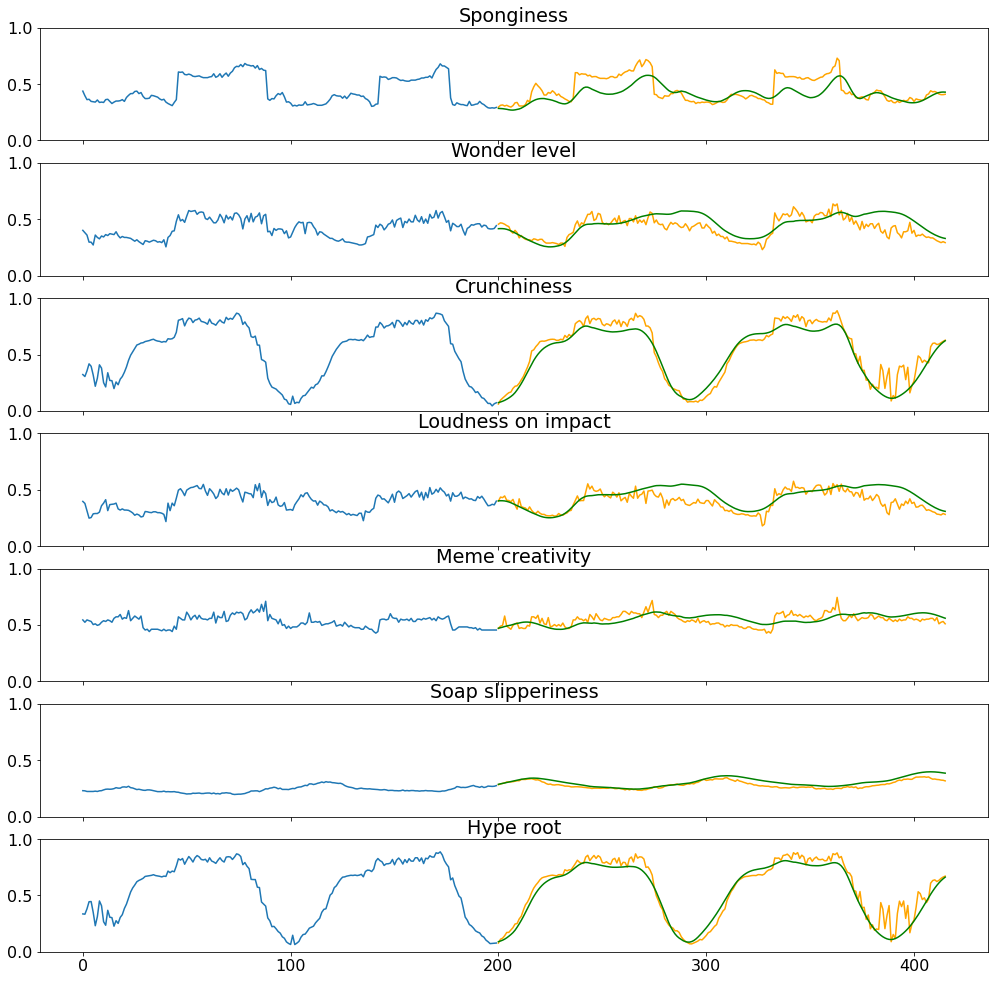
\includegraphics[width=\linewidth]{pics/pred_attention.png}
    \caption{Encoder/Decoder with Luong attention}
\end{figure}

\section{Conclusions}
In this report we presented our small journey in the world of time series forecasting with 
neural network architectures. Starting from the basic memory blocks we built and evaluated 
several models, spacing between different architectures.
We expected the encoder/decoder with attention to be our best performing model but,
due to our implementation (we think we might have overcomplicated things a little bit),
the simpler 3-layer BiLSTM model showed the best results; despite this, we had the chance to 
see first-hand how powerful the attention mechanism can be and why it is such a big deal.

\newpage
\section*{Appendix A: \textit{BiLSTM} model}
\begin{figure}[h]
    \centering
    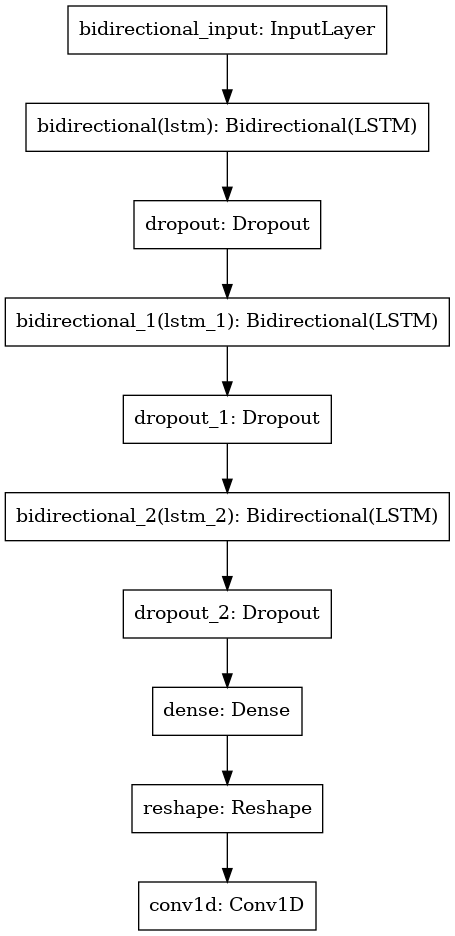
\includegraphics[width=0.8\linewidth]{pics/bilstm_model.png}
    \caption{Encoder/Decoder with Luong attention}
\end{figure}
\vfill\break
\section*{Appendix B: \textit{attention} model}
\begin{figure}[h]
    \centering
    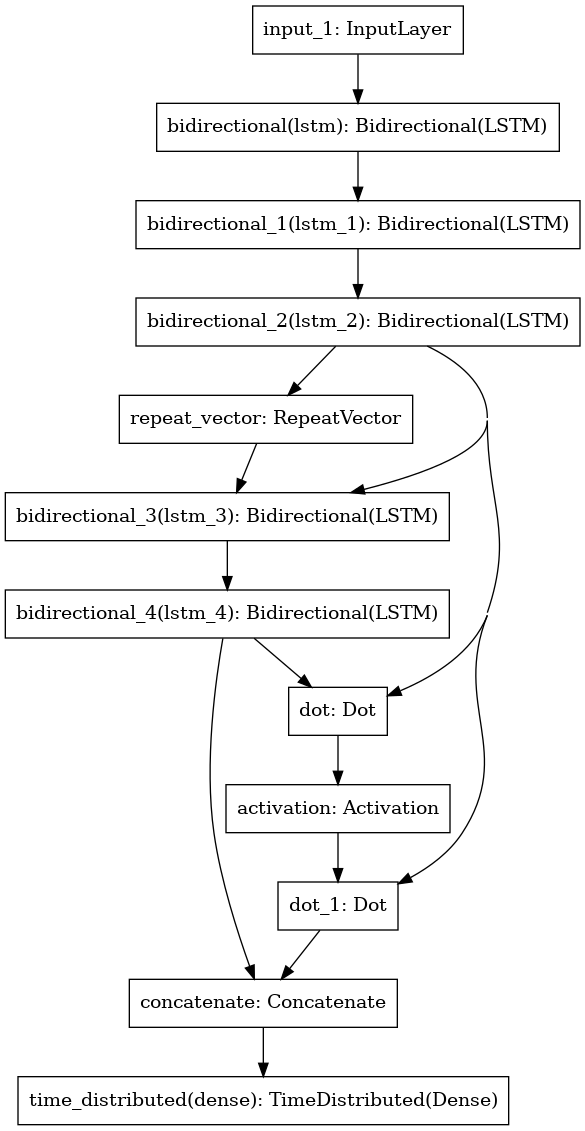
\includegraphics[width=0.8\linewidth]{pics/attention_model.png}
    \caption{Encoder/Decoder with Luong attention}
\end{figure}
For the sake of clarity, we omitted the dropout layers; it is
important to note that without dropout this model is way too overfit, scoring a RMSE of 32.68 on the 
secret test set.



\end{document}